\documentclass{article}
\usepackage{pgfplots}
\pgfplotsset{compat=1.18}

\begin{document}
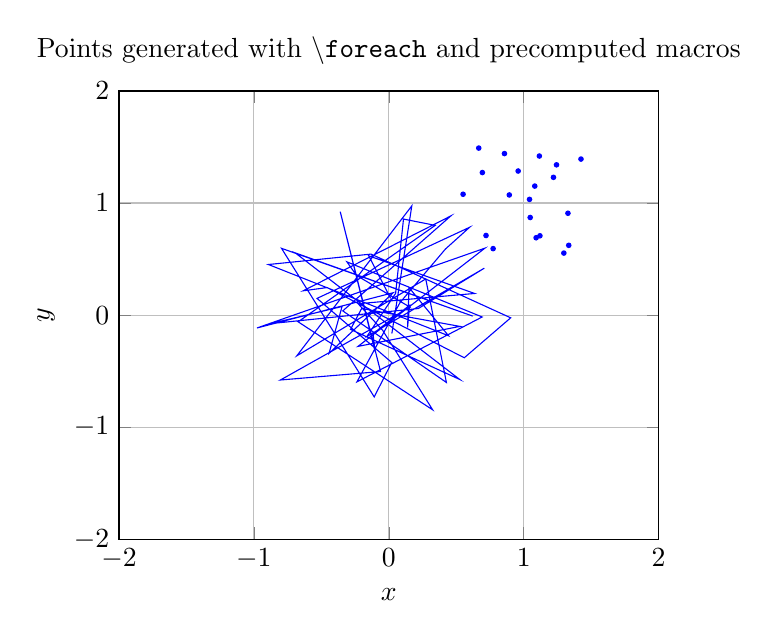
\begin{tikzpicture}
  \begin{axis}[
    xmin=-2, xmax=2, ymin=-2, ymax=2,
    xlabel=$x$, ylabel=$y$, grid=major,
    title=Points generated with \texttt{\textbackslash foreach} and precomputed macros
  ]
    \pgfmathsetseed{42} % reproducible
    \foreach \i in {1,...,20} {%
      \pgfmathsetmacro{\x}{(rand/2+1)}%
      \pgfmathsetmacro{\y}{(rand/2+1)}%
      \addplot[only marks, mark=*, blue, mark size=0.8pt] coordinates {(\x,\y)};%
    }

%    \foreach \i in {1,...,60} {%
%      \pgfmathsetmacro{\theta}{rand*360}%
%      \pgfmathsetmacro{\r}{(exp(-4 * pow(rand,2))}%
%      \pgfmathsetmacro{\x}{\r*cos(\theta)}%
%      \pgfmathsetmacro{\y}{\r*sin(\theta)}%
%      \addplot[only marks, mark=*, blue, mark size=0.8pt] coordinates {(\x,\y)};%
%    }
    
    % Initialize empty coordinate list
    \edef\coordlist{}

    \foreach \i in {1,...,60} {
      \pgfmathsetmacro{\theta}{rand*360}
      \pgfmathsetmacro{\r}{exp(-2 * pow(rand,2))}
      \pgfmathsetmacro{\x}{\r*cos(\theta)}
      \pgfmathsetmacro{\y}{\r*sin(\theta)}
      \xdef\coordlist{\coordlist (\x,\y)}
    }

    % Plot all points as a connected path
    \addplot[blue, thin] coordinates {\coordlist};

  \end{axis}
\end{tikzpicture}
\end{document}